\documentclass[a4paper,12pt]{scrartcl}

\usepackage[utf8]{inputenc}
\usepackage[ngerman]{babel}
\usepackage{cite} 
\usepackage{graphicx}
\usepackage[sort=use]{glossaries}
\usepackage[colorlinks=true, urlcolor=black, linkcolor=black, citecolor=black]{hyperref}
\graphicspath{{img/}}
\usepackage{xcolor}
\newcommand\todocomment[1]{\textcolor{red}{#1}}
%\renewcommand\todocomment[1]{}


\makeglossary
\newglossaryentry{JourneyPlanner}
{
	name={JourneyPlanner},
	description={Ein JourneyPlanner ist eine Software welche Verbindungsdaten analysiert und daraus die bessten reisewege von einem Punkt zu einem anderen berechnen kann.},
} 



\begin{document}
	
	\todocomment{Hund ist nicht Katze}
	\title{BA ÖV Journey Planning}
\subtitle{Implementation des Connection Scan Algorithmus}
\date{August 4, 2018}
\author{ Christian Bühler \and Flavio Tobler}

\maketitle
	\newpage
	\pagenumbering{Roman}
	\newpage
	\section{Abstract}
\label{abstract}
In dieser Arbeit geht es darum Unterkünfte anzuzeigen die in der Nähe von Attraktionen sind. Das Problem ist alleine durch die Luftliniendistanz können gewisse Orte als fälschlicherweise nahe eingestuft werden. Um dieses Problem zu Lösen verwendet man Fahrplandaten des Öffentlichen Verkehrs und ein Algorithmus der diese Aufgabe löst. Hieraus wird ein Journey-Planner entwickelt der diese Aufgabe lösen soll.
\newline
\newline
Für die Umsetzung werden zuerst die zur Verfügung stehenden Datensätze erläutert und auf deren Vor-/Nachteile eingegangen. Anschliessend werden die bekannten Algorithmen vorgestellt und analysiert. Zusätzlich werden aber auch Optimierungsmöglichkeiten aufgezeigt.
\newline
\newline
Am Ende dieser Arbeit wird erklärt weshalb man sich für diese Datensätze bzw. diesen Algorithmus entschieden hat um den Journey-Planner zu entwickeln.

	\newpage
	\tableofcontents
	\newpage
	\pagenumbering{arabic}
	\newpage
	\printglossaries
	\newpage
	
	
	\section{Einleitung}
Einleitung: Nutzen und Sinn des Projektes + Grobe Kapitelübersichtsbeschreibung der Arbeit
	
	\section{Augabenstellung}
\todocomment{Unsere BA Aufgabenstellung}
\label{AufgabenstellungBA}
\begin{itemize}
	\item Schreiben sie eine Implementation des CSA für den OpenTripPlanner. Dieser muss OTP-Development-Richtklinien konform sein.
	\item Implementieren sie die Schweizer GTFS und OpenStreetMap daten für den OTP, so dass Punkt zu Punkt Verbindungen in der Schweiz berechnet werden können.
	\item Implementieren sie den Schweizer realtime GTFS-Feed, so dass das Programm auf Verspätungen oder Fahrplanänderungen reagieren kann.
	\item Implementieren sie Skalierungsoptimierungen für das Programm, so dass es mit einem landesweiten System bessere Performanz liefert.
	\item Führen sie Performance Tests durch und vergleichen sie das Implementierte System mit dem auf Dijkstra basierenden OTP.
	\item Dokumentieren sie ihre Ergebnisse und schreiben sie einen ausführlichen Bericht.
\end{itemize}

\subsection{Lastenheft}
\label{Lastenheft}
\begin{tabular}{ | p{5cm} | l | l | }
	\hline
	\multicolumn{3}{|c|}{Funktionale Anforderungen} \\
	\hline
	Anforderung & Anforderungsart & Priorisierung \\
	\hline
	Der CSA muss als Berechnungsalgorithmus verwendet werden. & Muss & 1 \\
	\hline
	Es kann eine Verbindung zwischen 2 Stationen zu einem bestimmten Zeitpunkt errechnet werden. & Muss & 2 \\
	\hline
	Fusswege zu Stationen hin können miteinbezogen werden können. & Muss & 3 \\
	\hline
	Das Programm kann auf Verspätungen und Fahrplanänderungen reagieren. & Muss & 4 \\
	\hline
	Mehrere mögliche Verbindungen können angezeigt werden. & Muss & 5 \\
	\hline
	Fusswege zwischen verschiedenen Stationen können miteinbezogen werden. & Soll & 6 \\
	\hline
	Die Angezeigte Route soll den Fahrlinien, z.B. Schienen, folgen. & Kann & 7 \\
	\hline
\end{tabular}
\newline
\newline
\newline
Nicht funktionale Anforderungen
\begin{itemize}
	\item Der Programmcode muss den OTP-Development-Richtlinien entsprechen.
	\item Die Query-Zeit muss weniger als 1 Sekunde betragen.
	\item Die Preprocessing-Zeit muss weniger als 30 Minuten betragen.
	\item Die Query-Zeit soll schneller als die des originalen OTP sein.
\end{itemize}
	
	\section{Ausgangslage}
Um unsere Programm und unser Vorgehen besser zu verstehen, müssen wir zuerst das von uns verwendete Basisprogramm sowie den von uns verwendeten Basisalgorithmus erläutern.

\subsection{JourneyPlanning}
Ein \hypertarget{JourneyPlanner}{JourneyPlanner} ist ein Programm, welches den optimalen Weg für eine Reise zwischen zwei oder mehr Orten findet. Im Gegensatz zum RoutePlanning oder Routenplanner bezieht sich ein JourneyPlanner nur auf öffentliche Verkehrsmittel und nicht auf Privatfahrzeuge.

\subsection{OpenTripPlanner}

Der \hypertarget{OTP}{OpenTripPlanner} \cite{otp}\footnote{\url{https://opentripplanner.org/}}, kurz OTP, ist eine auf der \gls{Maven-Repository} 
aufbauende Trip-Planning Software. Er war anfangs für Städte ausgelegt, findet nun jedoch auch in ersten landesweiten Verkehrsnetzen Anwendung. Er wurde von einem OpenSource-Kollektiv aus mehr als 100 Personen in acht Jahren entwickelt. \newline

Der OTP basiert auf dem A*-Algorithmus und verwendet GTFS-Daten und OpenStreetMap-Daten. In einem Preprocessing-Schritt wird der Graph für den Algorithmus erstellt. Dieser kann in einer Datei gespeichert werden oder direkt im RAM des Servers gelagert werden. Während des Betriebs kann der Graph angepasst werden, so dass das Programm auf verspätete Züge reagieren kann. \newline

Der OTP erzeugt für jeden Aufruf eine neue Instanz des Graphen. Dies ist nötig, weil während des Aufrufs Daten im Graphen verändert werden, diese sich jedoch nicht auf andere Aufrufe auswirken dürfen.

OTP steht unter einer \gls{GNU Lesser General Public License}. 


\subsection{Verwendung des OpenTripPlanners}
Der OTP wird über das OTPMain-File im Packet org.opentripplanner.otp gestartet. Dabei benötigt er drei Parameter. Mit den Parameter \texttt{--build} wird dem OTP ein Pfad mitgegeben, in welchem die GTFS- und OSM-Daten abgelegt sind. Mit dem Parameter \texttt{--inMemory} behält der OTP seine Daten ausschliesslich im RAM. Wird der Parameter nicht angegeben, so werden die Daten im im Build-Parameter angegebenen Pfad gespeichert. \newline

Mit einem weiteren Parameter kann festgelegt werden, wie viel Arbeitsspeicher das Programm maximal verwenden darf. Der Parameter lautet \texttt{-Xmx4g}. Die Zahl steht dabei für die Anzahl der zur Verfügung gestellten Gigabyte.


\subsection{Dijkstra-Algorithmus}
Der \hypertarget{dij}{Dijkstra-Algorithmus} \cite{dij_bell} ist ein auf einem Graphen basierender Wegfindungsalgorithmus. Er bildet einen Graph, wobei Haltestellen Punkte sind und Verbindungen die Linien zwischen den Punkten. Alle Verbindungen besitzen eine Gewichtung, welche mit der benötigten Zeit korreliert. Der Algorithmus sucht nun den Weg mit der geringsten summierten Gewichtung vom Start- zum Zielpunkt.

\subsection{A* Algorithmus}
Der \hypertarget{A*}{A*-Algorithmus} \cite{dij_a} ist eine Erweiterung des Dijkstra-Algorithmus. Er durchsucht den Graphen nicht in alle Richtungen sondern sucht gezielt in die Richtung des Zielpunktes. Dadurch lässt sich die Performance verbessern.

\subsection{Connection Scan Algorithmus}
Der \hypertarget{CSA}{Connection Scan Algorithm} \cite{csa} , kurz CSA,  ist ein moderner Algorithmus zur Bearbeitung von Anfragen auf zeitplanbasierten Sytemen. Er basiert, im Gegensatz zu den gängigen Algorithmen wie z.B. dem Dijkstra-Algorithmus, nicht auf einem gewichteten Graphen. \newline

Es gibt zwei Arten des CSA. Zum einen den EAS (EarliestArrivalConnectionScan) welcher die frühestmögliche Ankunftszeit und wenn benötigt auch noch den dazugehörigen Journey zurückliefert. Zum anderen den PCS (ProfileConnectionScan) welcher alle möglichen Journeys berechnet und den besten Journey nach mehreren Kriterien sortieren kann. Beide sind darauf ausgelegt genau einen Journey zurückzugeben. \newline

Der Algorithmus iteriert über eine nach Abfahrtszeit sortierte Liste aller Verbindungen. Dabei werden vom Start- oder Zielpunkt erreichbare Verbindungen markiert. Dadurch entsteht ein Netz aus Verbindungen, welches sich immer weiter aufspannt. Dies wird dann so lange wiederholt, bis ein Weg zwischen den beiden Punkten gefunden wurde. Danach gibt der Algorithmus entweder die früheste Ankunftszeit am Zielpunkt oder den besten Weg vom Startpunkt zum Zielpunkt zurück.




 

\subsection{General Transit Feed Specification}
%Erklärung was GTFS ist und was dessen aufbau und regeln sind
\hypertarget{GTFS}{General Transit Feed Specification (GTFS)}\cite{gtfsinhalt}\cite{gtfs} ist ein von Google entwickeltes Dateiformat zum Austausch von öffentlichen Verkehrsdaten sprich Fahrpläne. Die Daten werden von der SBB-Platform\footnote{\url{https://opentransportdata.swiss/}} zur Verfügung gestellt. GTFS ist ein statisches Dateiformat und beinhaltet keine Echtzeitdaten wie Verspätungen, Ausfälle etc. und wird deshalb auch GTFS-Static genannt. Die Daten werden in verschiedenen Textfiles zur Verfügung gestellt, welche wiederum viele wichtige Informationen enthalten. GTFS-RT(RealTime) ist eine Erweiterung der GTFS-Static-Daten. Dies ermöglicht es die GTFS-Daten dynamisch zu aktualisieren. \cite{gtfs-rt-google} \newline

\begin{tabular}{|l|c|l|}  \hline
	Dateiname & Pflicht? & Definition \\ \hline
	agency.txt & ja & Geschäftsstellen, die Daten zur Verfügung stellen \\ \hline
	stops.txt & ja & Haltestellen mit ihrer Position \\ \hline
	routes.txt & ja & Verkehrsverbindungen (Linien) mit den Fahrzeugarten \\ \hline %(zeitunabhängig)
	trips.txt & ja & Fahrten  \\ \hline												%(zeitabhängig)
	stop\_times.txt & ja & Zeiten, in der Fahrzeuge ankommen/abfahren an Haltestellen \\ \hline
	calendar.txt & ja & Fahrplanveränderungen (Jahreszeiten) \\ \hline
	calendar\_dates & optional & Ausnahmeplan für bestimmtes Datum \\ \hline
	fare\_attributes.txt & optional & Fahrpreise und die Art der Bezahlung \\ \hline
	fare\_rules.txt & optional & Fahrpreisregeln verschiedener Zonen  \\ \hline
	shapes.txt & optional & Beschreibt den Weg eines Fahrzeuges (Darstellung) \\ \hline
	frequencies.txt & optional & Fahrpläne ohne fixe Stopp-Zeiten. \\ \hline
	transfers.txt & optional & Umsteigpunkte verschiedener Routen (Linien) \\ \hline
	feed\_info.txt & optional & Zusätzliche Informationen über den Datensatz \\ \hline	
\end{tabular}

%\cite{gtfsInhalt} %Verweis aus Fachmodul!!
Daten, die bisher nicht von der Plattform zur Verfügung gestellt werden: fare\_attributes.txt, fare\_rules.txt, frequencies.txt.



	
	\section{Methode}
\todocomment{Evaluationen usw.}

\subsection{Performance Test (Benchmarking)}

\subsection{Verzeichnisstruktur}
Da der OTP sehr viele verschiedene Pakete besitzt haben wir uns entschieden alles was den CSA betrifft und von uns programmiert wird in einem separaten Paket zu sammeln wie in Abbildung \ref{fig:csapackage} zu sehen. Dadurch behalten wir die Übersicht was wir zusätzlich in das bestehende Programm hinzugefügt haben. 

\begin{figure}[h]
	\centering
	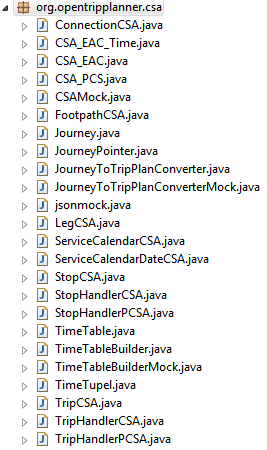
\includegraphics[width=5cm]{img/csapackage.png}
	\caption{Dieses Bild gibt eine Übersicht welche Klassen in unserem Paket vorhanden ist.}
	\label{fig:csapackage}
\end{figure}

Da ein Stop aus der Library gleich bei uns heissen würde. Führt dies zu einem Namenskonflikt mit der Klasse Stop für den CSA und Stop von der onebusaway Library. Ein weiterer Namenskonflikt war Leg diese Klasse ist schon im OTP(Grundversion) vorhanden.
Um dieses Problem zu lösen benannten wir die Klassen, die wir benötigen werden für den CSA um. Indem wir die Klassen mit der CSA Endung erweiterten z.B. Stop in StopCSA.\newline

\subsection{Zeitplan}

\subsection{Mocking}
Das Programm kann grob in drei Abschnitte aufgeteilt werden. Das erstellen des Zeitplans aus den GTFS-Daten, den Wegfindungsalgorithmus und einen Converter welcher das Resultat in die von der Webseite verlangte Form bringt. Damit diese drei Abschnitte separat behandelt werden können und das Programm dennoch jederzeit überprüft werden kann entschieden wir uns ein Mockup für die Abschnitte durchzuführen.



	
	\section{CSA für OTP}

\subsection{Datenstruktur}
Der CSA benötigt zwei Datenstrukturen. Eine Zeittafel(TimeTable) für die Eingabe von Daten und eine Reise(\texttt{Journey}) für die Rückgabe von Daten. 

\subsubsection{Zeittafel (\texttt{TimeTable})}
Der \texttt{TimeTable} ist eine Zeittafel die alle benötigen Daten für den CSA zur Verfügung stellt. Die Datenstruktur ist ein Quadrupel aus Sammlungen von Fusswege(\texttt{FootpathCSA}), Haltestellen(\texttt{StopCSA}), Verbindungen(\texttt{ConnectionCSA}) und Fahrten(\texttt{TripCSA}).\newline 
Neben den \texttt{.add()} und \texttt{.show()} Funktionen für die Sammlungen enthält die \texttt{TimeTable}-Klasse die Methode \texttt{.getFootpathChange()} welche für eine Haltestelle die Umsteigzeit zurückgibt.

\begin{figure}[htb]
	\centering
	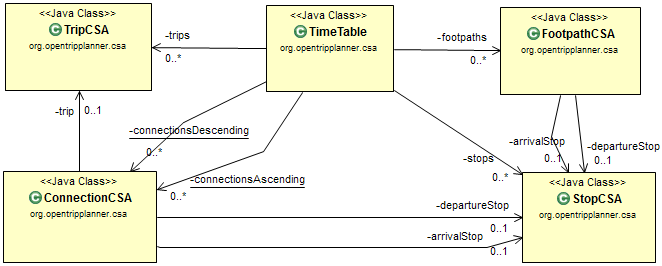
\includegraphics[width=8cm]{img/TimeTable.png}
	\caption{Hier ist das UML-Diagramm zur \texttt{TimeTable} Datenstruktur zu sehen.}
	\label{fig:uml-timetable}
\end{figure}

\subsubsection{Fusswege (\texttt{FootpathCSA})}
\begin{figure}[htb]
	\centering
	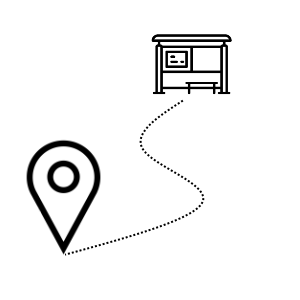
\includegraphics[width=5cm]{img/footpath.png}
	\caption{Symbolbild für den Fussweg(FootpathCSA)}
	\label{fig:footpath}
\end{figure}
Ein Fussweg kann zwei verschiedene Funktionen haben. Er besteht aus einem DepartureStop, einem ArrivalStop sowie einer Dauer. Wenn der DepartureStop und der ArrivalStop gleich sind repräsentiert der Footpath einen Umsteigeprozess. Wenn sie unterschiedlich sind repräsentiert er einen Laufweg zu einem Stop hin oder von einem Stop weg.


\subsubsection{Haltestellen (\texttt{StopCSA})}
\begin{figure}[htb]
	\centering
	
\includegraphics[width=5cm]{img/stop.png}
	\caption{Symbolbild für die Haltestelle(StopCSA)\cite{stop-pic}}
	\label{fig:stop}
\end{figure}
Ein Stop ist eine Haltestelle für öffentliche Verkehrsmittel. Ein Stop besitzt einen Namen, Längen- und Breitengrad. 

\subsubsection{Verbindungen (\texttt{ConnectionCSA})}
\begin{figure}[htb]
	\centering
	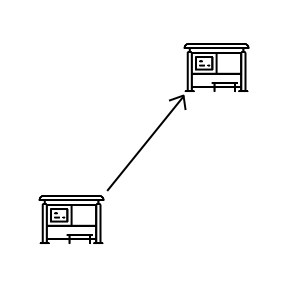
\includegraphics[width=5cm]{img/connection.png}
	\caption{Symbolbild für die Verbindung(ConnectionCSA)}
	\label{fig:connection}
\end{figure}
Eine Connection ist eine Verbindung zwischen einem DepartureStop und einem ArrivalStop . Die Connection hält Daten wie die Abfahrtszeit vom DepartureStop und die Ankunftszeit vom ArrivalStop. Zudem weiss die Connection zu welchem Trip sie gehört. 

\subsubsection{Fahrten (\texttt{TripCSA})}
\begin{figure}[htb]
	\centering
	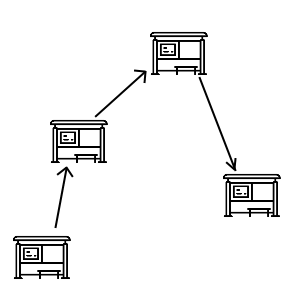
\includegraphics[width=5cm]{img/trip.png}
	\caption{Symbolbild für die Fahrt(TripCSA)}
	\label{fig:trip}
\end{figure}
Als Trip wird die Fahrt eines Öffentlichen-Verkehrsmittels von der Start-Station bis zur End-Station bezeichnet. Es ermöglicht den CSA ohne umsteigen erreichbare Orte zu erkennen. Ein Trip besteht aus mehreren Connections die aneinandergereiht sind. Des weiteren hält der Trip Informationen über das Verkehrsmittel(Zug,Bus usw.) und welche Geschäftsorganisation dieses Verkehrsmittel zur Verfügung stellt. Ausserdem enthält der Trip Informationen ob der Trip an jenem Tag auch fährt oder nicht.

\subsection{Reise (\texttt{Journey})}
Ein Journey ist ein vom CSA berechneter Weg vom Start- zum Zielpunkt. Er besteht aus einem StartPath, welcher den Fussweg zur ersten Station hin darstellt, sowie eine Liste aus journeyPointern welche den Weg mit allen Umsteigestationen repräsentiert. 
\begin{figure}[htb]
	\centering
	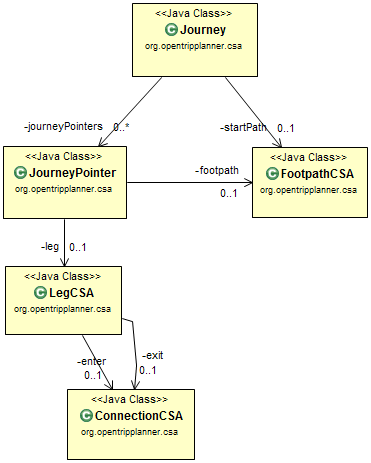
\includegraphics[width=8cm]{img/Journey.png}
	\caption{Hier ist das UML-Diagramm zur \texttt{Journey} Datenstruktur zu sehen.}
	\label{fig:uml-journey}
\end{figure}

\subsubsection{Reisezeiger (\texttt{JourneyPointer})}
Ein JourneyPointer ist eine Hilfskonstruktion welche der CSA anlegt um die berechnete Abfolge von Stationen später wieder rekonstruieren zu können.Ein JourneyPointer besteht aus einem Leg sowie einem Footpath. Dabei handelt es sich beim Leg um eine Fahrt in einem ÖV vom einsteigen bis zum Aussteigen und beim Footpath um das darauffolgende Umsteigen oder das erreichen des Ziels.

\subsubsection{Fahrtabschnitte (\texttt{LegCSA})}
Ein Leg ist die Fahrt in einem Öffentlichen Verkehrsmittel vom einsteigen bis zum aussteigen. Dies ermöglicht es den Journey nicht von Station zu Station, sondern von Umsteigen zu Umsteigen zu rekonstruieren. Ein Leg besteht aus einer EnterConnection und einer ExitConnection. 

\subsection{Programmablauf}
\begin{figure}[htb]
	\centering
	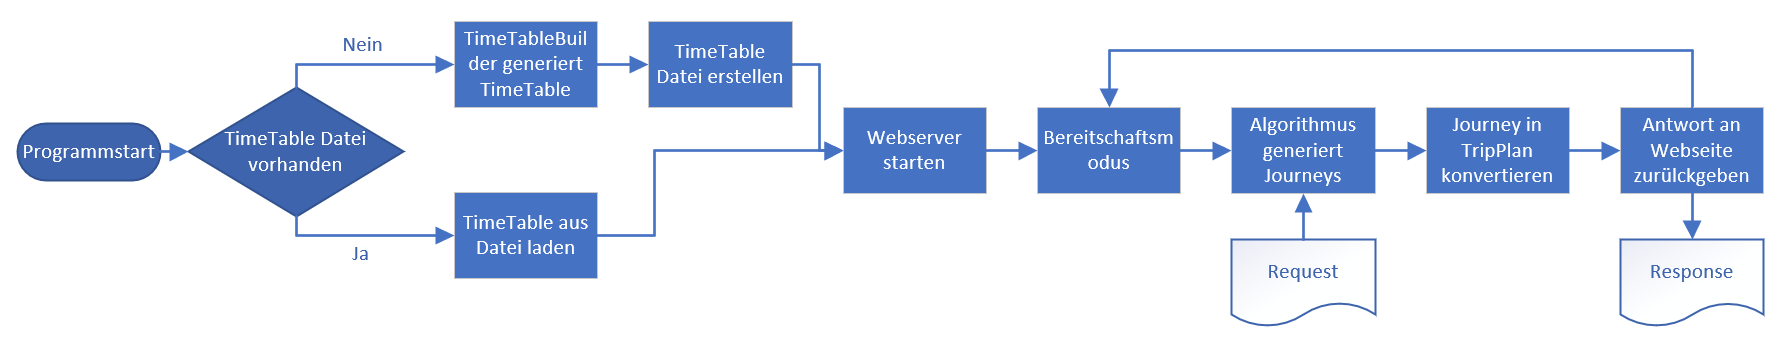
\includegraphics[width=15cm]{img/programmablauf.png}
	\caption{Programmablauf des OTP mit dem CSA}
	\label{fig:programmablauf}
\end{figure}

\subsubsection{Zeittafelerzeuger (\texttt{TimeTableBuilder})}
Da wir für den CSA eine Zeittafel (\texttt{TimeTable}) benötigen, muss diese durch den Zeittafelerzeuger (\texttt{TimeTableBuilder}) erstellt werden. Die zugrundeliegenden GTFS-Daten können jedoch nicht in dieser Form einfach der Zeittafel übergeben werden. Der Zeittafelerzeuger erzeugt die Zeittafel. Durch die Funktion \texttt{.loadFromGtfs()} werden die Daten eingelesen und in die benötigte Form gebracht. Dieser Prozess kann durchaus einige Zeit in Anspruch nehmen. Deshalb wird nachdem die Zeittafel fertig befüllt wurde anschliessend serialisiert und als Java-SerializedObjectFile gespeichert. Somit brauchen wir nicht mehr jedesmal die Zeittafel komplett neu einzulesen und zu erstellen. Durch die Funktion \texttt{.loadFromSerializedObjectFile()} kann die zwischengespeicherte Zeittafel jederzeit eingelesen werden, was die Zeit um eine schon in Form gebrachte Zeittafel zu erzeugen um einiges verkürzt. Unabhängig von beiden Methoden wird dann der Server gestartet.

\subsubsection{Server}
Der Server wird über die Main-Funktion gestartet. Bei dem Server handelt es sich um einen \texttt{GrizzlyServer}.Der Server stellt eine Webseite zur Verfügung(Webserver). Über diese Webseite kommuniziert der Server mit allen Clients, indem es alle Requests(Anfragen) entgegen nimmt und alle dazugehörigen Responses(Antworten) zurückschickt. Die Kommunikation läuft hierbei über ein HTTP-Protokoll zwischen Server und Clients(Browser). 

\begin{figure}[htb]
	\centering
	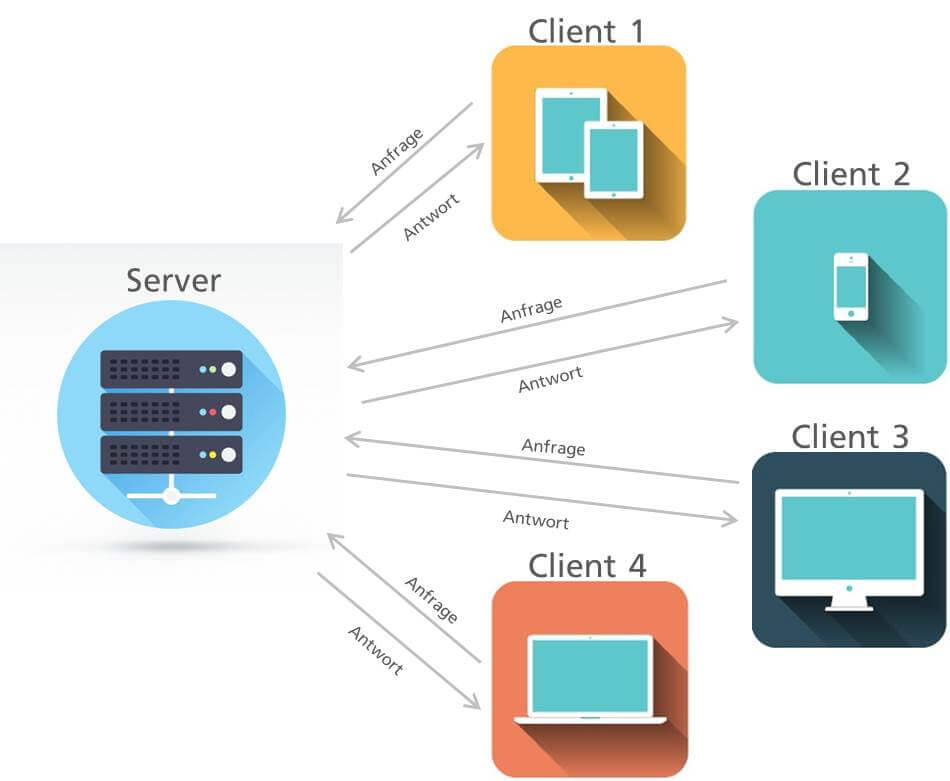
\includegraphics[width=8cm]{img/serverrequestresponse.jpg}
	\caption{Darstellung der Kommunikation zwischen Clients und Server\cite{server-pic}}
	\label{fig:serverrequestresponse}
\end{figure}




\subsubsection{Webseitenaufruf}
Wenn ein Aufruf von der Webseite eingeht so wird die plan Methode der Klasse PlannerResource aufgerufen. Diese erhält die Anfragenparameter in einem \texttt{RoutingRequest}-Objekt. Das im Preprocessing generierte TimeTable-Objekt wird als neue Instanz übergeben. Dies wird gemacht, da der OTP eine seperate Isntanz des Algorithmus für jeden Aufruf verwendet. Der TimeTable sowie der Request werden dann der \texttt{createJourneys}-Methode des Algorithmuses übergeben. Dessen Rückgabe wird in einem Set von Journeys gespeichert.


\subsubsection{Earliest Arrival Connection Scan}
Der Earliest Arrival Connection Scan Algorithmus\cite{csa}, kurz EACS, ist ein Wegfindungsalgorithmus welcher MEAT (Minimum Expected Arrival Time) Problem löst. Er sucht sich den schnellsten Weg vom Start zum Zielpunkt und beendet dann seine suche ohne nach Alternativen zu suchen. 

Er arbeitet mit einer nach Abfahrtszeit sortierten Liste von Verbindungen. Über diese iteriert er dann aufsteigend wobei als Startpunkt die erste Verbindung, welche nach der im Request spezifizierten Abfahrtszeit abfährt. 

Jede Verbindung wird auf drei Eigenschaften überprüft:
\begin{itemize}
	\item Ist der Abfahrtsort der Startort?
	\item Wurde der Abfahrtsort schon von einer früheren Verbindung erreicht?
	\item Wurde das zur Verbindung gehörende Fahrzeug schon von einer früheren Verbindung benutzt?
\end{itemize}
Wenn eine dieser drei Bedingungen erfüllt ist so wird dies im Ankunftsort der Verbindung mit einem Zeiger auf den Ort, bei welchem man in das jeweilige ÖV eingestiegen ist, vermerkt. Der Ort bei welchem man eingestiegen wird mithilfe eines \texttt{Trip-Bits} gespeichert. Wenn eine ÖV zum ersten mal verwendet wird so wird der Startort gespeichert und das \texttt{Trip-Bit} wird für das ÖV gesetzt. Wird das ÖV erneut verwendet so ist das \texttt{Trip-Bit} bereits gesetzt und der Startort wird nicht überschreiben. 

Sobald der Algorithmus eine Verbindung findet, welche eine der drei Bedingungen erfüllt und gleichzeitig der Ankunftsort dem Zielort entspricht, hat er einen Journey zum Ziel gefunden. Die Schleife wird unterbrochen und der Algorithmus baut sich vom Zielort aus mithilfe der Zeiger den kompletten Journey auf welcher dann als Antwort zurückgegeben wird.

Alternativ kann der ECSA auch nur die früheste Ankunftszeit anstelle des kompletten Journeys zurückgeben. In dieser Version müssen keine Zeiger gespeichert werden, was den Algorithmus schneller macht. Es gehen jedoch Informationen über den Reiseweg verloren.

\subsubsection{Profile Connection Scan}
Der Profile Connection Scan Algorithmus\cite{csa}, kurz PCS, ist ein Wegfindungsalgorithmus welcher alle möglichen Reisen in einem bestimmten Zeitraum errechnet und sich anschliessend nach den gewünschten Kriterien die  beste Reise zurückgibt.

Er arbeitet auch mit einer nach Abfahrtszeiten sortierten Liste von Verbindungen. Im Gegensatz zum EACS iteriert er absteigend über die Verbindungen. Er sucht also die Verbindung vom Zielpunkt aus. Jede Verbindung durchläuft dabei drei Prüfungen:

\begin{itemize}
	\item Kommt man ans Ziel wenn man aussteigt?
	
	Diese Bedingung überprüft ob der Ankunftsort der Verbindung der Zielort des Requests ist. Ist dies der Fall, so wird im Abfahrtsort der Verbindung die Ankunftszeit sowie die dazugehörige Verbindung gespeichert. Zusätzlich wird die Ankunftszeit für das jeweilige öffentlichen Verkehrsmittels gespeichert.
	\item Kommt man ans Ziel wenn man umsteigt?
	
	Es wird überprüft ob vom Ankunftsort der Verbindung schon ein Weg gefunden wurde, welcher zum Zielort führt. Dazu wird überprüft, ob im Ankunftsort eine Ankunftszeit gespeichert wurde. Ist dies der Fall so wurde schon ein möglicher Weg vom Ankunftsort zum Zielort gefunden. Dann werden die Informationen wie in der ersten Bedingung im Abfahrtsort und dem öffentlichen Verkehrsmittel gespeichert.
	\item Kommt man ans Ziel wenn man sitzen bleibt?
	
	Es wird überprüft, ob von diesem öffentlichen Verkehrsmittel aus schon eine Weg zum Zielort gefunden wurde. Dazu wird überprüft ob für das öffentlichen Verkehrsmittel schon eine Ankunftszeit gespeichert wurde. Ist dies der Fall so werden die Informationen wie in den ersten beiden Schritten im Abfahrtsort und dem öffentlichen Verkehrsmittel gespeichert.
\end{itemize}
Die Suche ist abgeschlossen sobald die Abfahrtszeit der Verbindung früher als die im Request definierte Abfahrtszeit ist. 

Nun wird vom Startpunkt aus jede gespeicherte Ankunftszeit überprüft. Dann wird von der zur Ankunftszeit gehörigen Verbindung der Ankunftsort genommen. Von diesem Ort aus werden wieder die gespeicherten Ankunftszeiten überprüft und die gleichen Schritte erneut durchgeführt. Dies wird so lange wiederholt bis der Ankunftsort der Zielort ist. Der gefundene Weg entspricht dann einem Journey zum Ziel. Der beste gefundene Journey kann dann als Response zurückgegeben werden. 
\subsubsection{JourneyToTripPlanConverter}
Die vom Algorithmus gefundenen Journeys werden dann zusammen mit dem Request der \texttt{generatePlan}-Methode des \texttt{JourneyToTripPlanConverter} übergeben. Dieser wandelt die Journeys in ein \texttt{TripPlan}-Objekt um, welches von der Webapplikation als Response erwartet wird.

Die vom Request benötigten Informationen werden zu beginn in das \texttt{TripPlan}-Objekt übertragen. Danach wird aus jedem Journey ein \texttt{Itinerary}-Objekt erzeugt. Dieses wird dann mithilfe der dem Journey zugehörigen \texttt{JourneyPointer} befüllt. Für die \texttt{Legs} sowie die \texttt{Footpaths} der \texttt{JourneyPointer} wird ein \texttt{Leg} generiert. Dies ist jedoch ein \texttt{Leg}-Objekt und kein \texttt{LegCSA}-Objekt. Während des ersten Durchlaufs wird zudem aus dem StartPath des Journeys ein Leg generiert. Dazu gibt es die beiden Methoden \texttt{legFromLeg()} und \texttt{legFromFootpath()}. Diese übertragen die benötigten Parameter und erstellen eine Geometrische-Form welche dem Fahrtweg folgen und für die Anzeige auf der Webseite benötigt werden. Wenn ein \texttt{Leg} aus einem \texttt{Footpath} generiert wird, wird zusätzlich überprüft ob dieser eine Distanz überwindet oder ob der Start- und Zielpunkt gleich sind. Dies dient dazu Umsteigewege hinauszufiltern, welche von der Webseite nicht als Leg benötigt werden, jedoch trotzdem in die Zeit mit einfliessen. Sobald alle \texttt{JourneyPointer} abgearbeitet sind wird das \texttt{Itinerary} den \texttt{TripPlan} hinzugefügt. Nachdem die 3 besten Journeys konvertiert wurden wird der \texttt{TripPlan} an die Webseite zurückgegeben.

	
	\section{Produkt}

\subsection{OTP mit Schweizer Daten implementieren}
Der originale OTP muss mit den Schweizer GTFS-Daten funktionieren, da er als Grundlage für den Algorithmus dient und einen Performancevergleich zwischen den beiden Algorithmen gemacht werden muss. Es gab zwei Probleme, welche dabei behandelt werden mussten.
\newline


Die SBB beschreibt in ihren GTFS-Daten einige Verbindungen mit dem Routentyp 1700 «Miscelaneous». Dieser Typ wird jedoch vom OTP nicht unterstützt da er nicht zugeordnet werden kann. Nach einer Überprüfung der SBB Daten stellte sich heraus, dass der Routentyp 1700 nur für einige Sessellifte sowie Autoverladestationen verwendet wird. Da diese beide nicht in unserem Scope liegen können sie ignoriert werden. Dazu fügten wir dem OTP einen Handler für den Routentyp 1700 hinzu welcher ihn als Auto definiert, da auch das Auto ausserhalb unseres Scpes liegt, jedoch vom OTP unterstützt wird.
\newline


Das zweite Problem war der benötigte Arbeitsspeicher. Für die Grafberechnung mit den SBB GTFS-Daten benötigt der OTP ca. 15 GB Arbeitsspeicher. Die von uns benötigten Rechner konnten diese Speichermenge jedoch nicht zur Verfügung stellen. Deshalb wird für die Berechnung mit den grossen Datensätzen ein Laborcomputer der HTW verwendet. Dieser entspricht mit seinen 32GB Arbeitsspeicher den Anforderungen.


\subsection{Kann OTP ohne .osm file ausgeführt werden?}
Das .osm steht für OpenStreetMap und ist eine Plattform\footnote{\url{https://www.openstreetmap.org/}} die frei nutzbare Daten(sprich Geodaten) zur Verfügung stellt. Wie z.B. Strassen, Wege, Gebäude, Haltestellen usw. OTP kann ohne .osm file ausgeführt werden. Jedoch werden dann keine Fusswege mit einberechnet um zu einer Haltestelle zu gelangen, wie man in Abbildung \ref{fig:ohneosmfile} erkennen kann.
Aber wenn OTP mit dem .osm File ausgeführt wird lässt sich anhand der Informationen einen Gehweg zu der Haltestelle finden (inklusive Laufzeit und Distanz), wie man in Abbildung \ref{fig:mitosmfile} erkennen kann. 

\begin{figure}[htb]
	\centering
	\begin{minipage}{0.45\linewidth}
		\centering
		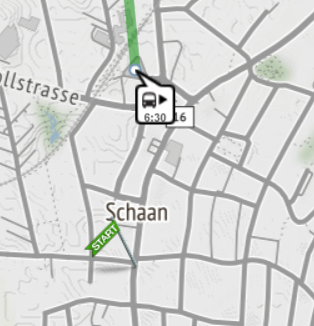
\includegraphics[width=6cm]{img/ohneosmfile.png}
		\caption{ohne .osm File}
		\label{fig:ohneosmfile}
	\end{minipage}
	%\hfill
	\begin{minipage}{0.45\linewidth}
		\centering
		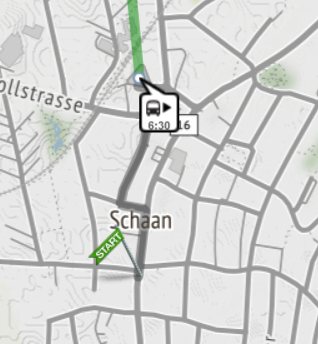
\includegraphics[width=6cm]{img/mitosmfile.png}
		\caption{mit .osm File}
		\label{fig:mitosmfile}
	\end{minipage}
\end{figure}


\subsection{Modellierung der Datenstrukur}
\todocomment{Java container klassen + UML Diagramm}

\subsection{Automatische generierte Klassendiagramme}
Klassendiagramme können sehr behilflich sein bei der Entwicklung. Sie geben einen Überblick welche Klassen miteinander agieren.
Der Opentripplaner besteht aus unzähligen verschiedenen Klassen. Um eine bessere Übersicht zu erhalten erzeugten wir mit dem Programm objectaid\footnote{\url{http://www.objectaid.com/home}} (ein Plugin für Eclipse) fast vollautomatisch Klassendiagramme. 

%beispielbild eines Klassendiagramms mit objectaid ?

\subsection{Dummy-GTFS Daten erstellen}
Wir haben selbst GTFS-Daten erstellt, weil ein komplettes Schweizer-GTFS schon ein paar Stunden braucht um die Daten einzulesen. So brauchen wir nicht bei jedem Ausführen des Programms jedes mal ein paar Stunden zu warten, was uns bei der Entwicklung viel Zeit erspart. Dadurch das wir dieses GTFS-Daten selber erstellt haben, wissen wir nun was genau vorhanden ist und können dadurch nachvollziehen ob z.B. Die GTFS-Daten richtig eingelesen wurden und daraus auch weitere Methoden auf ihre Richtigkeit Überprüfen kann.\newline

Das Dummy-GTFS wurde anhand der bestehenden Schweizer-GTFS Daten erstellt. Im Schweizer-GTFS sind auch die Daten des öffentlichen Verkehrs von Liechtenstein enthalten. Wir haben uns entschieden nur ein Teil der Liechtensteinischen Busverbindungen zu übernehmen und selber zu erstellen um den Inhalt der Schweizer-GTFS Daten beizubehalten.

\begin{figure}[h]
	\centering
	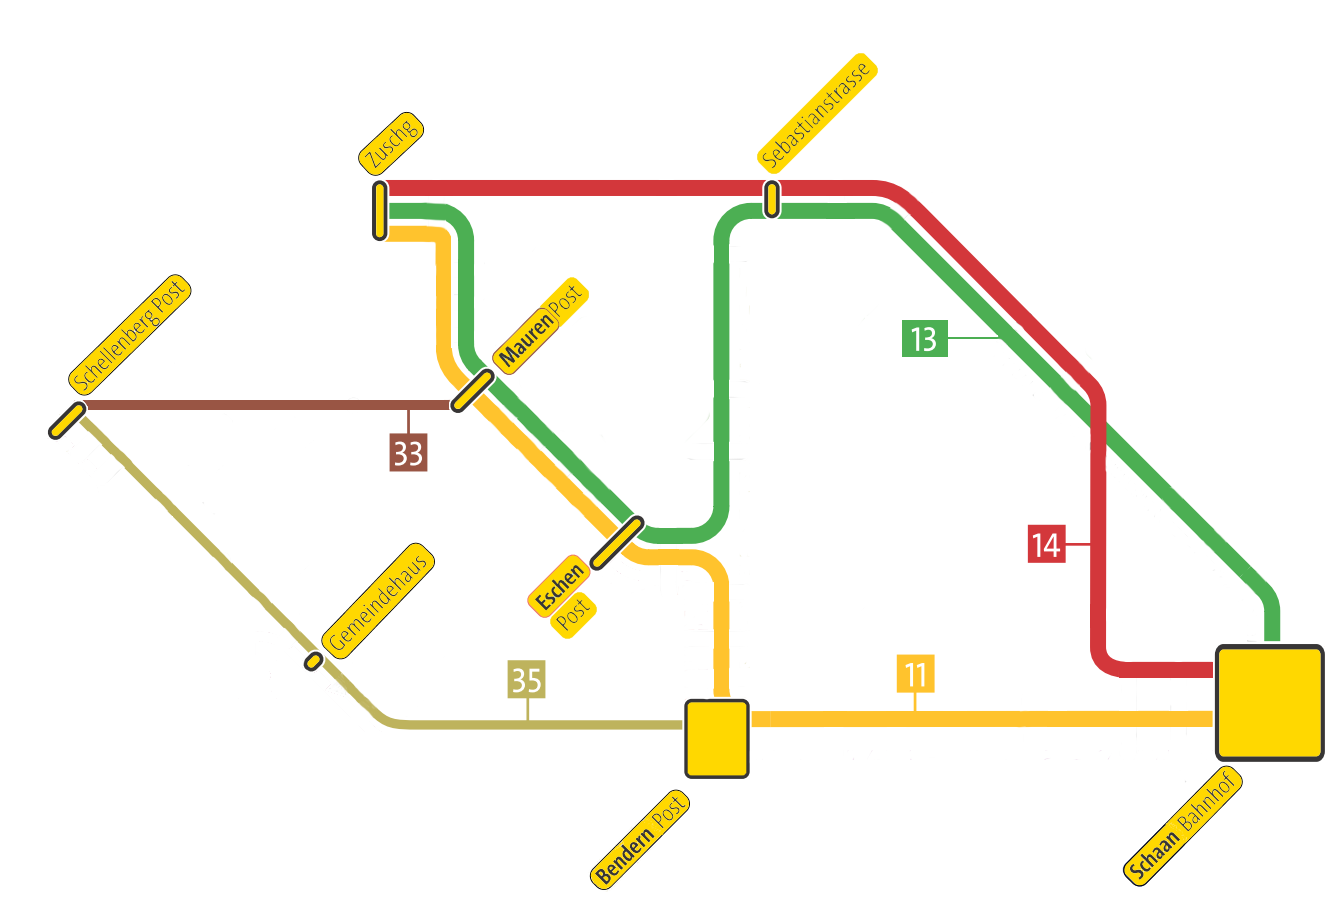
\includegraphics[width=12cm]{img/LiniennetzDummyGTFS.png}
	\caption{Dieses Bild gibt eine Übersicht welche Haltestellen und Routen im Dummy-GTFS vorhanden ist.}
	\label{fig:DummyGTFS-uebersicht}
\end{figure}

\subsection{Mocking}
Das Programm kann grob in drei Abschnitte aufgeteilt werden. Das erstellen des Zeitplans aus den GTFS-Daten, den Wegfindungsalgorithmus und einen Converter welcher das Resultat in die von der Webseite verlangte Form bringt. Damit diese drei Abschnitte separat behandelt werden konnten und das Programm dennoch jederzeit überprüft werden konnte entschieden wir uns ein Mockup für die Abschnitte durchzuführen.

\subsubsection{CSAMock}
Das Mocking des CSA bekommt ein Zeitplan-Objekt als Eingabe und speichert dieses zur Kontrolle in einem JSON-File. Danach wird manuell ein Journey erstellt welches eine Reise von «Heerbrugg, Dornacherhof» nach «Heerbrugg, Bahnhof» repräsentiert. Diese Verbindung wurde gewählt, da es eine einfache Busfahrt ohne Zwischenstops ist. Dieser Journey wird dann als Antwort zurückgegeben.

\subsubsection{TimeTableBuilderMock}
Das Mocking des TimeTableBuilders erstellt manuell einen Zeitplan mit zwei Haltestellen und einer Busverbindung. Dieser wird anschliessend als Response zurückzugeben.

\subsubsection{JourneyToTripPlanConverterMock}
Der als Parameter bekommene Journey wird zur Überprüfung in ein JSON-File gespeichert. Anschliessend wird manuell eine Webseitenantwort aufgebaut. Anfangs wurde eine Reise ohne Zwischenstops, Umsteigen und Fusswege zurückgegeben. Doch in folgenden Schritten wurde das Mocking erweitert um die zuvor erwähnten, komplexeren Fälle zu behandeln.

\subsection{TimeTableBuilder}
Die Aufgabe des TimeTableBuilder ist es Daten aus dem GTFS zu lesen und anschliessend eine Datenstruktur daraus zu erzeugen die der Connection Scan Algorithm benötigt. Zum einlesen der GTFS-Daten wird die Onebusaway Library verwendet. Diese erzeugt anhand der Daten Objekte.Die Objektdaten von der Onebusaway Library sind in Listen abrufbar.
z.B. Entspricht im GTFS Stop.txt ein Zeileneintrag einem Stop Objekt. Durch diese Library ist es einfacher Daten aus dem GTFS abzufragen. z.B. von einem Stop kann man gezielt nach dem Namen fragen\texttt{stop.getName()}.\newline  

Da ein Stop aus der Library gleich bei uns heissen würde. Führt dies zu einem Namenskonflikt mit der Klasse Stop für den CSA und Stop von der onebusaway Library. Um dieses Problem zu lösen benannten wir die Klassen, die wir benötigen werden für den CSA um. Indem wir die Klassen mit der CSA Endung erweiterten z.B. Stop in StopCSA.\newline

Durch diese Library lässt es sich nun relativ einfach die Daten aus dem GTFS lesen und anschliessend mit den gewünschten Daten die benötigten Objekte erstellen.Dafür wir die Funktion \texttt{.loadFromGtfs()} ausgeführt.  Stop, Footpath und Trips lassen sich relativ leicht erstellen weil die GTFS-Daten hierbei schon in sehr ähnlich Form aufgebaut sind. Jedoch ist es bei der Connection etwas schwieriger, da die Daten nicht in dieser Art direkt vorhanden sind. Die Connections müssen beim der Stop\_times.txt immer zwei hintereinanderfolgende Einträge(Objekte) vergleichen um zu Erkennen das es sich um eine Connection handelt. Eine Connection wird erkannt wenn sie auf den selben Trip stattfinden und die stop\_sequence Zahl muss grösser sein als der vorhergehende Eintrag. Wenn dieser Fall nur Zutrifft wurde eine Connection erkannt. Bevor jetzt aber das Connection Objekt einfach erzeugt werden kann müssen noch die richtigen Referenzen gefunden werden. Den die Stops und Trips wurden zuvor schon erzeugt. Den eine Connection muss wissen auf welchem Trip sie ist und welche Departure- und ArrivalStops sie enthält. Nachdem also eine Connection gefunden wurde wird er richtige Trip in der bestehenden Liste gesucht, anhand der TripId kann der Trip aus der Liste gefunden werden. Das selbe geschieht auch mit den Departure- und ArrivalStops. Wenn alle Informationen gefunden wurden wird das Connection Objekt erzeugt und in das TreeSet(sortiere Liste) übergeben. Durch die \texttt{.compareTo()} Funktion der Connection lässt sie sich an der richtigen Stelle im TreeSet einfügen. Somit bekommen wir alle Connections sortiert nach der Departuretime. Am Ende der Funtion wird ein Java-SerializedObjectFile vom TimeTable erstellt. Somit wird das gewünschte Format zwischengespeichert. Das erstellen dieser Datei benötigt nur 1-2 Minuten und die Datei ist 367MB gross.\newline

Die Funktion \texttt{.loadFromGtfs()} benötigt etwa 60h um das Schweizer GTFS einzulesen. Aber durch Optimierung konnte die Zeit veringert werden auf 22h. Indem wir die nicht mehr einfach wie vorher ständig nach dem Trip wieder suchen wenn eine Connection gefunden wurde. Durch zwischenspeichern der Referenz des vorhergehenden Trips kann dieser wiederverwendet werden, wenn die TripId der Einträge übereinstimmen. Somit muss nur ein Trip in der Liste gesucht werden wenn diese TripId nicht übereinstimmen. Zudem kann durch zwischenspeichern der Referenz auf den vorhergehenden Stop eine Suche in der Liste vermieden werden. Da ein Trip und Stop nur einmal vorkommt in der Liste, kann beim durchlaufen mit einer Suchschleife die suche nach dem Trip vorzeitig abgebrochen werden, was verhindert das unnötig weiter nachdem Trip/Stop gesucht wird.  

Die Funktion \texttt{.loadFromSerializedObjectFile()} kann verwendet werden um zwischengespeicherte TimeTables einzulesen. Das SerializedObjectFile das zuvor aus dem Schweizer GTFS erstellt wurde lässt sich innerhalb von 151s einlesen.


\subsection{JourneyToTripPlanConverter}
Der JourneyToTripPlanConverter bildet einen von der Webseite benötigten TripPlan aus den vom CSA generierten Journeys. Aus dem Mocking sind die benötigten Parameter schon bekannt so dass die Generierung nun nur noch automatisiert werden muss. Dabei gab es jedoch mehrere Punkte welche speziell beachtet werden mussten.
\begin{enumerate}
	\item Ein Journey besitzt nur eine Dauer für den kompletten Weg. Der TripPlan jedoch speichert sich separate Werte für Fahrzeit, Laufzeit und Wartezeit. Die Fahrzeit und die Laufzeit können dabei einfach aus den Start- und Stop-Zeiten der Legs oder Footpaths übernommen werden. Bei der Wartezeit beseht jedoch das Problem das sie den Zeitunterschied zwischen zwei Abschnitten repräsentiert. Dies bedeutet, dass in der Schleife die beiden zu vergleichenden Zeiten nicht gleichzeitig vorhanden sind. Dieses Problem wird umgangen indem die Endzeit des Itinerarys nach jedem berechneten Leg angepasst wird. Somit stimmt dieser Wert immer mit der Endzeit des Legs des vorhergehenden Schleifendurchgangs überein. 
	\item Jedes Leg im TripPlan benötigt ein LegGeometry-Object. Dies wird benötigt damit die Webseite eine Linie entlang des Fahrtweges anzeigen kann. Dies wird mithilfe der GeometryUtils-Bibliothek und den Start- und Endkoordianten eine Gerade erstellt. Diese 
	\item Im TripPlan wird ein Fussweg mithilfe von verschiedenen WalkSteps definiert. Diese benötigen jedoch eine Variable AbsoluteDirection welche 8 Himmelsrichtungen repräsentiert. Diese musste in einer komplexen Winkelberechnung aus den Koordinaten berechnet werden. Danach wird der Winkel auf 45 Grad Abschnitte gerundet und den jeweiligen Himmelsrichtungen zugeordnet.
	\item Der CSA stellt sowohl Fusswege als auch Umsteigeprozesse als Footpaths dar. Umsteigeprozesse werden aber vom TripPlan nicht dargestellt, ausser das sie in die Zeitberechnung miteinfliessen müssen. Daher müssen die Fusswege und Umsteigeprozesse unterschieden werden. Nachdem ein Leg generiert wurde, jedoch noch bevor es der Liste von Legs hinzugefügt wurde, wird überprüft, ob die Start- und Zielkoordianten gleich sind. Ist dies der Fall so handelt es sich um einen Umsteigeprozess und das berechnete Leg wird der Liste nicht hinzugefügt. Die berechneten Zeiten werden jedoch trotzdem für das nächste Leg verwendet.
\end{enumerate}

\subsection{ConnectionScanAlgorithm}
Von den beiden CSA-Versionen kümmerten wir uns zuerst um den Earliest Arrival Scan Algorithmus, da dieser weniger Komplex ist und als Grundlage für den Profile Connection Scan Algorithmus dient.
\subsubsection{EAS}
Am Anfang werden für alle Stops und Trips Handler angelegt. Handler sind Hilfskonstruktionen welche alle informationen der Stops und Trips beinhalten, welche im verlauf der Berechnung geändert werden müssen wie zum Beispiel die EinstiegsConnection für die Trips. Das ist nötig, da wir mit einem persistenten TimeTable-Objekt arbeiten welches für die nächsten Anfragen nicht verändert werden darf.
\newline


Danach werden die Zeitvariabeln vorbereitet. Das Jahr, der Monat und der Tag müssen aus dem Request übernommen werden, da die Zeitangaben des Zeitplans nur auf die Uhrzeit und nicht auf das Datum beziehen. Dazu werden die Datumswerte in Variablen gespeichert.  Nun wird im Stop-Handler des Startstops die Startzeit des Requests eingetragen. Für alle anderen Stop-Handler wird die zeit auf den 31.12.20000 gesetzt. Diese Zeit simuliert eine Unendlich grosse Zahl welche trotzdem noch mit den Calendar-Methoden verglichen werden kann.
\newline


Dann werden alle aufsteigend nach Abfahrtszeit sortierten Connections durchlaufen. Für jede Connection wird überprüft, ob die im Stop-Handler des Startstops der Connection gespeicherte Zeit vor der abfahrtszeit der Connection ist, oder ob im zur Connection passenden Trip-Handler das Trip-Bit gesetzt ist. Das Trip-Bit ist am Start auf «false» gesetzt. Sobald eine Connection gefunden wird welche eine der zwei vorherigen Bedingungen erfüllt so wird es für den zur Connection passenden Trip auf True gesetzt. Damit werden sich erreichbare Verkehrsmittel gemerkt, so dass weitere Connections im gleichen ÖV auch als erreichbar markiert sind. Die zweite Bedingung prüft ob der Startstop der Connection schon erreicht wurde. Anfangs ist nur die Zeit im Stop-Handler des Startstops gesetzt. Alle anderen Zeiten sind auf Unendlich gesetzt. Somit werden nur Connections behandelt welche vom Startstop ausgehen und später abfahren als die im Request definierte Startzeit. Sobald so eine Connection gefunden wurde wird die Ankunftszeit in den Stop-Handler des Ankunftsstops der Connection geschrieben. Somit ist nun auch dieser als erreichbar markiert und wird bei weiteren Durchläufen beachtet. Zusätzlich wird jedesmal wenn eine Connection gefunden wurde ein JourneyPointer im Stophandler des Ankunftsstops der Connection gespeichert, um den Journey später rekonstruieren zu können.
\newline


Das Breakkriterium für die Schleife ist wenn die Abfahrtszeit der Connection später ist als die im Stop-Handler des Zielstops gespeicherte Zeit. Diese Zeit ist auf Unendlich gesetzt und wird erst neu gesetzt wenn ein Journey zum Zielpunkt gefunden wurde. Da die Connections aufsteigend nach Abfahrtszeit durchlaufen werden ist dies auch automatisch die am Frühesten ankommende Reise. 
\newline


Nun wird vom Zielstop aus der Journey rekonstruiert. Im JourneyPointer des Zielstops steht der zuvor erreichte Stop. Nun wird der JourneyPointer dieses neuen Stops untersucht. Dies wird so lange wiederholt bis der Startstop erreicht ist. Nun werden die gefundenen Stops in umgekehrter Reihenfolge in den Journey eingetragen und der Journey wird zurückgegeben.
\subsubsection{PCS}
Der Profile Connection Scan Algorithmus erstellt am Anfang auch Stop- und Triphandler sowie die im EAS erwähnten Zeitvariabeln. Danach werden die Verbindungen in einer Schleife durchlaufen. Im Gegensatz zum EAS werden sie jedoch absteigend nach Abfahrtszeit durchlaufen. Damit jedoch nur ein Zeitfenster der Verbindungen um die gesuchte Zeit herum behandelt werden muss wird vor der Schleife ein EAS durchgeführt, welcher nur die früheste Ankunftszeit zurückliefert. Dieser Zeit werden dann zwei Stunden hinzugerechnet und sie wird als Einstugspunkt für die Schleife benutzt. 
\newline


Nun werden drei Zeitvariablen gesetzt. Die erste zeigt wann und ob man ans Ziel kommt, wenn man aus dem ÖV aussteigt. Dies ist nur der Fall, wenn der Ankunftsort der Connection dem Zielort entspricht. In diesem Fall wird die Ankunftszeit der Connection in der Zeitvariable gespeichert. Ist dies nicht der fall so wird sie auf Unendlich gesetzt.
\newline


Die zweite Zeitvariable zeigt wann und ob man ans Ziel kommt, wenn man im ÖV sitzen bleibt. Dabei wird die TripZeit in der Zeitvariablen gespeichert. Ist diese ungleich unendlich so ist das Zeil mit weiterfahren erreichbar.
\newline


Die dritte Zeitvariable zeigt wann und ob man ans Ziel kommt, wenn man in ein anderes ÖV umsteigt. Dazu werden alle TimeTupels im Zielstop aufsteigend durchlaufen bis eine TimeTupel gefunden wurde, welches später abfährt als die Ankunftszeit der Connection plus die Umsteigezeit. Da jeder Stop ein default TimeTupel mit der Zeit Unendlich hat wird immer eine Möglichkeit gefunden. 
Danach werden die drei Zeitvariablen verglichen und der früheste wird behalten. Dies ist nun die schnellste Zeit in welcher man von dieser Connection aus das Ziel erreichen kann. Nun wird von der Abfahrtszeit der Connection die Umsteigzeit abgezogen und es wird mit diesen beiden Zeiten ein neues TimeTupel erstellt. Nun wird überprüft ob die Ankunftszeit nicht unendlich ist und somit der Zielort erreichbar ist. Wenn dies der Fall ist so wird das Tupel zusammen mit einen JourneyPointer in den Stop-Handler geschrieben, für den Trip wird eine TripZeit festgelegt und falls für diesen Trip noch keine ExitConnection festgelegt ist wird die aktuelle Connection eingetragen. Dies wird so lange wiederholt bis die Abfahrtszeit der Connection vor der im Request spezifizierten Startzeit ist.
\newline


Nun werden die Journeys vom Startstop aus rekonstruiert. Es wird ein Journey für jedes im Startstop gespeichertes TimeTupel generiert. Dabei wird erste JourneyPointer im Journey eingetragen. Dann werden die im Endstop des Journeys gespeicherten TimeTupels überprüft. Hierbei wird nur das erste Tupel und nicht alle verwendet. Diese Entscheidung wurde aus performance Gründen getroffen, da die Anzahl an schritten ansonsten Exponenziell ansteigen würde. Dies wird so lange wiederholt bis der Zeilstop erreicht ist. 
\newline


Der Vorgang benötigt jedoch noch einen Zusatz, da der Algorithmus auch Reisen findet, welche Kreise fahren und den selben Ort mehrfach anfahren. Um dies zu verhindern wird eine Liste mit allen schon angefahrenen Stops geführt. Für jeden neuen JourneyPointer wird geprüft ob der Ankuftsstop schon in der Liste vorhanden ist. Ist dies der Fall so wird ein Bit auf TRUE gesetzt. Am ende werden nur Journey der Rückgabe hinzugefügt bei welchen kein Stop mehrfach angefahren wurde.

\subsection{Performance-Test}
Um den Performance-Test durchzuführen wird ein JUNIT-Test mit der JUNIT-Benchmark erweiterung genutzt. Dieser führt mehrere Requests durch. Ein Reqeust ohne Umsteigen. Einer mit einmal Umsteigen und einer mit zweimal umsteigen.
\newline


Die Tests schlugen jedoch bei dem CSA ohne die QuadTree-Optimierung fehl, da die Anfrage mit den kompletten Schweizer-Daten länger als 24 Stunden dauerte.





	
	\section{Resultate}
Unsere Tests und deren Ergebnisse darstellen
	
	\section{Fazit}
Unsere Implementation des CSA im OTP ist funktionsfähig. Die von uns angestrebte Performance konnte jedoch nicht erreicht werden. Unsere Implementation ist mit den Schweizer GTFS-Daten um den Faktor 10000 langsamer als der Originalalgorithmus des OTP.

Der grösste Performanceverlust rührt von unserer implementation Der Stop- und Trip-Handler. Die Handler haben zwar eine Referenz auf das ihnen zugehörige Objekt, jedoch hat das Objekt keine Referenz zum Handler. Da in unserem Algorithmus jedoch mit den Objekten gearbeitet wird und dann im zum Objekt gehörigen Handler Informationen abgespeichert werden müssen, muss jedes mal mit einer Suchschleife der richtige Handler gefunden werden. Dies führt dazu, dass in einem Schleifendurchlauf des Algorithmus acht Suchschleifen durchlaufen werden, welche jeweils auch grosse Datensätze durchsuchen müssen. 

Um dieses Problem zu lösen müssten die Referenzen gedreht werden, so dass die Objekte auf ihre jeweiligen Handler referenzieren. Somit lassen sich die Suchschleifen vermeiden. Aus zeitlichen Gründen konnten wir diese Optimierung jedoch nicht mehr durchführen.


	
	\newpage
	\listoffigures
		\bibliography{test2,Programme}
	\bibliographystyle{IEEEtran}
	
	

	
	
	
	
	
\end{document}